\section{Manipulation: exploring the environments to learn}

\label{sect:manipulation}

IST has continued working on the acquisition and usage of affordance
knowledge (see Deliverable 1.6). The work has focused on two different
directions: (i) the extension of the Bayesian network model described
in Deliverable 1.6 for unsupervised learning of  affordances through
self-exploration; and (ii) the use of this knowledge in imitation
context to learn through observation.

\subsection{Affordance acquisition}
As described in previous documents, we have proposed a general
framework for affordance acquisition based on Bayesian networks. The
robot is able to build through exploration a network describing the
relations between its actions, the object features and the resulting
effects of the action. In the last months, we have completed the set
of experiments to validate the Bayes network affordance model. More
precisely, we have shown how extra features help to disambiguate
situations and improve the prediction capabilities of the
model. Figure~\ref{fig:manipulation:affordances}(a) shows the playground used in the experiments and
Figure~\ref{fig:manipulation:affordances}(b) shows the resulting network.

For instance, the difference of touch and tap on a ball is clear when
applied to objects that roll such as a ball. However, when tapping or
touching a box-like object, the resulting effects are the same. In
this case, it is important to add proprioceptive features such as
contact information to dissambiguate both cases. By using this
proprioceptive information, the robot is able to improve the model of
the world. Figure~\ref{fig:manipulation:affordances}(c) compares the action recognition ratio using a
model with contact information (Figure~\ref{fig:manipulation:affordances}(b)) and a model without this
information.
This work has been published in \cite{montesano:etal:2007}.

\begin{figure}
\begin{tabular}{ccc}
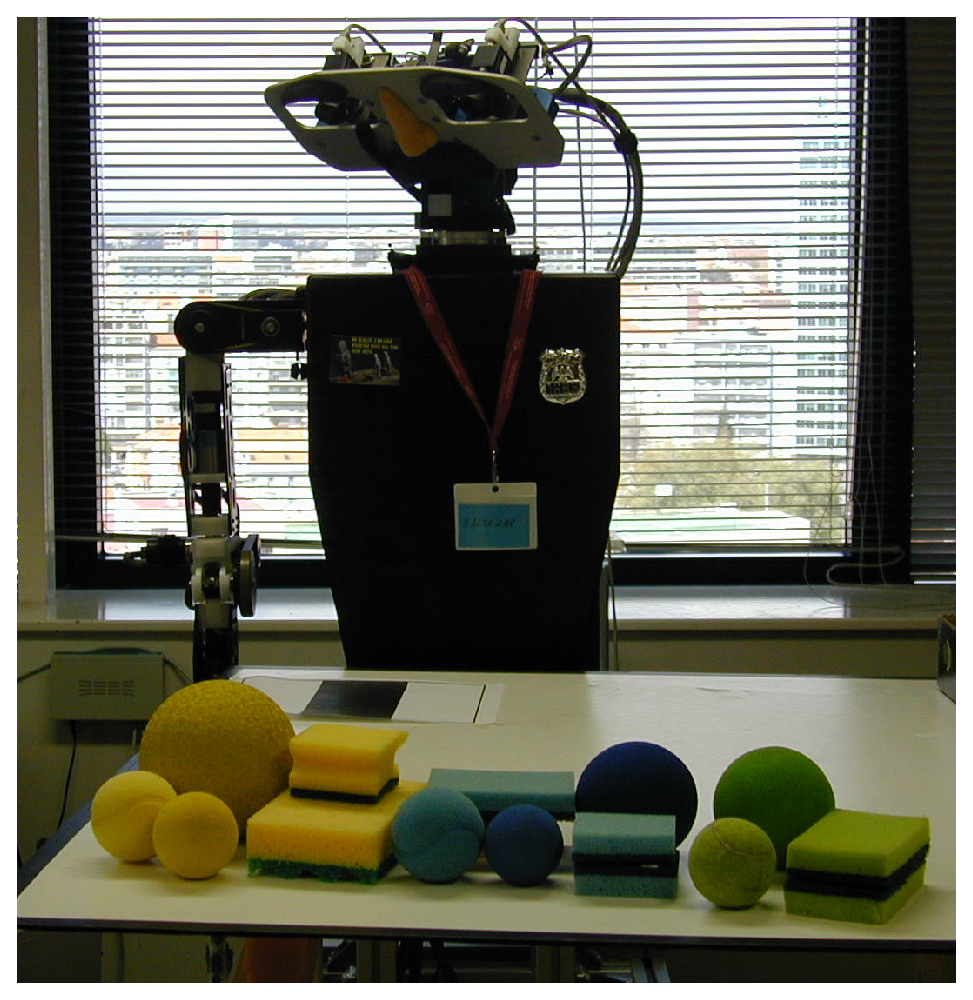
\includegraphics[width=0.3\columnwidth]{images/setup.eps} &
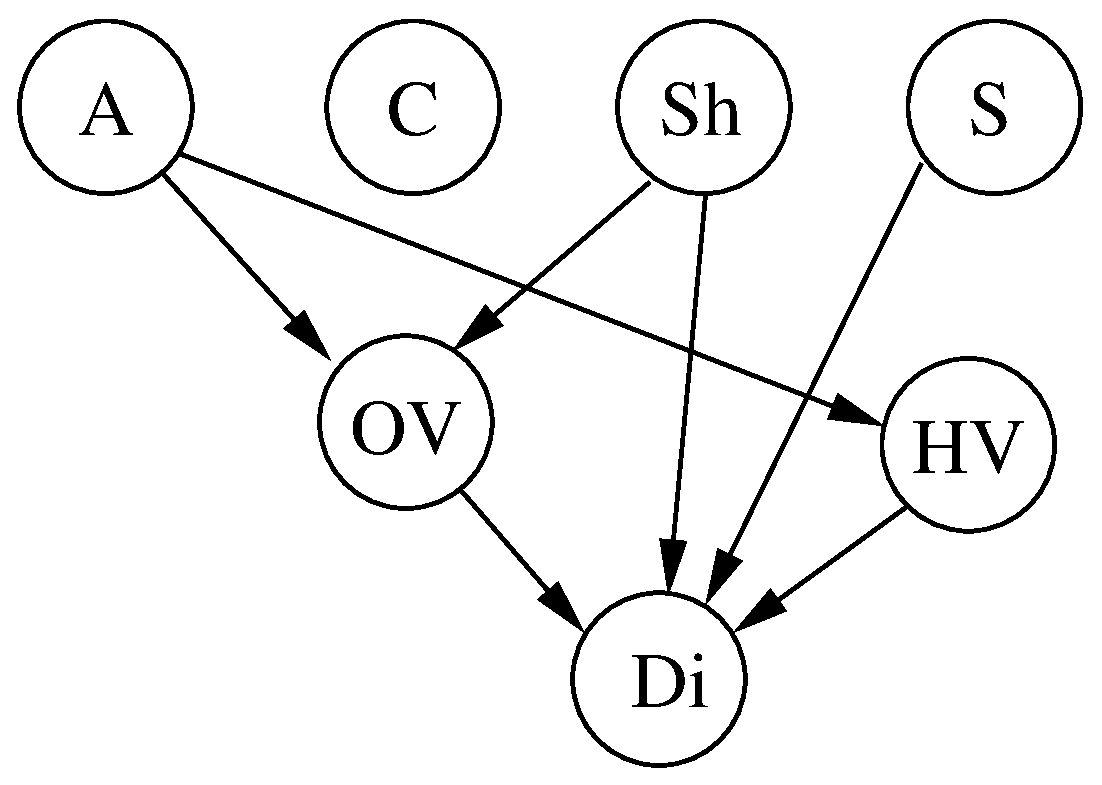
\includegraphics[width=0.3\columnwidth]{images/MCMCIROS1_p072.eps} &
\includegraphics[width=0.3\columnwidth]{images/resIROSActionRecog.eps} \\
(a) & (b) & (c) \\
\end{tabular}
% Figure 5
\caption{(a) Playground for affordance acquisition, (b) Affordance
  network learnt,  (c) ratio of action recognition w/o contact
  information.}
\label{fig:manipulation:affordances}
\end{figure}


\begin{figure}
\centering
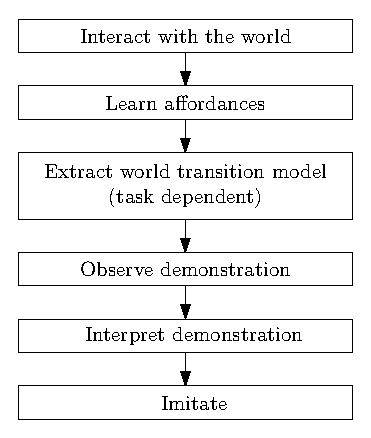
\includegraphics[width=0.3\columnwidth]{images/Diagram.eps}
%Figure 6
\caption{Path to imitation.}
\label{fig:manipulation:path}
\end{figure}

\subsection{Affordance based imitation}
The main objective of acquiring and modeling affordances is to provide
a general model of the world mechanisms in terms of robot actions and
perceptual skills. This model provides a sound base to develop more
complex behaviors. IST has started to explore the use of the
affordance model to develop imitation behaviors. The proposed
framework is shown in Figure\ref{fig:manipulation:path}. The robot
first learn the affordance network model. Then, it uses this model to
estimate a rough transition model for the proposed task , to extract
information from the demonstrations and translate them into its own
motion repertoire. Using Bayesian inverse reinforcement learning, the
robot interprets the demonstrations and extracts its own policy to
achieve the same goal.

We have conducted some experiments to evaluate the proposed methodology. The robot learnt how to sort different objects from a human demonstration (see Figure~\ref{fig:manipulation:experim}(a)).
 
It is important to note that the affordance model only provides a
rough estimate of the transition probabilities between the different
states of the task. In addition to this, the action recognition may
fail. We have done some preliminary studies on the impact of this
errors in the proposed
framework. Figure~\ref{fig:manipulation:experim}(b) shows the impact
of action recognition errors in the learn policy. Although more
studies are needed, the results suggests the proposed framework is
able to cope with the uncertainty and model errors.
%
This work has been published in \cite{montesano:etal:2007}.
\begin{figure}
\begin{tabular}{cc}
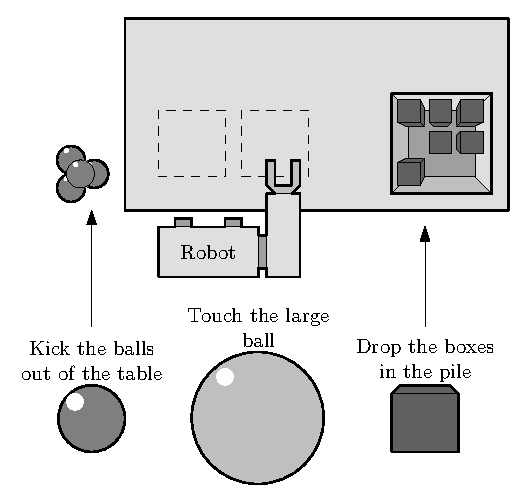
\includegraphics[width=0.45\columnwidth]{images/Recycler.eps} &
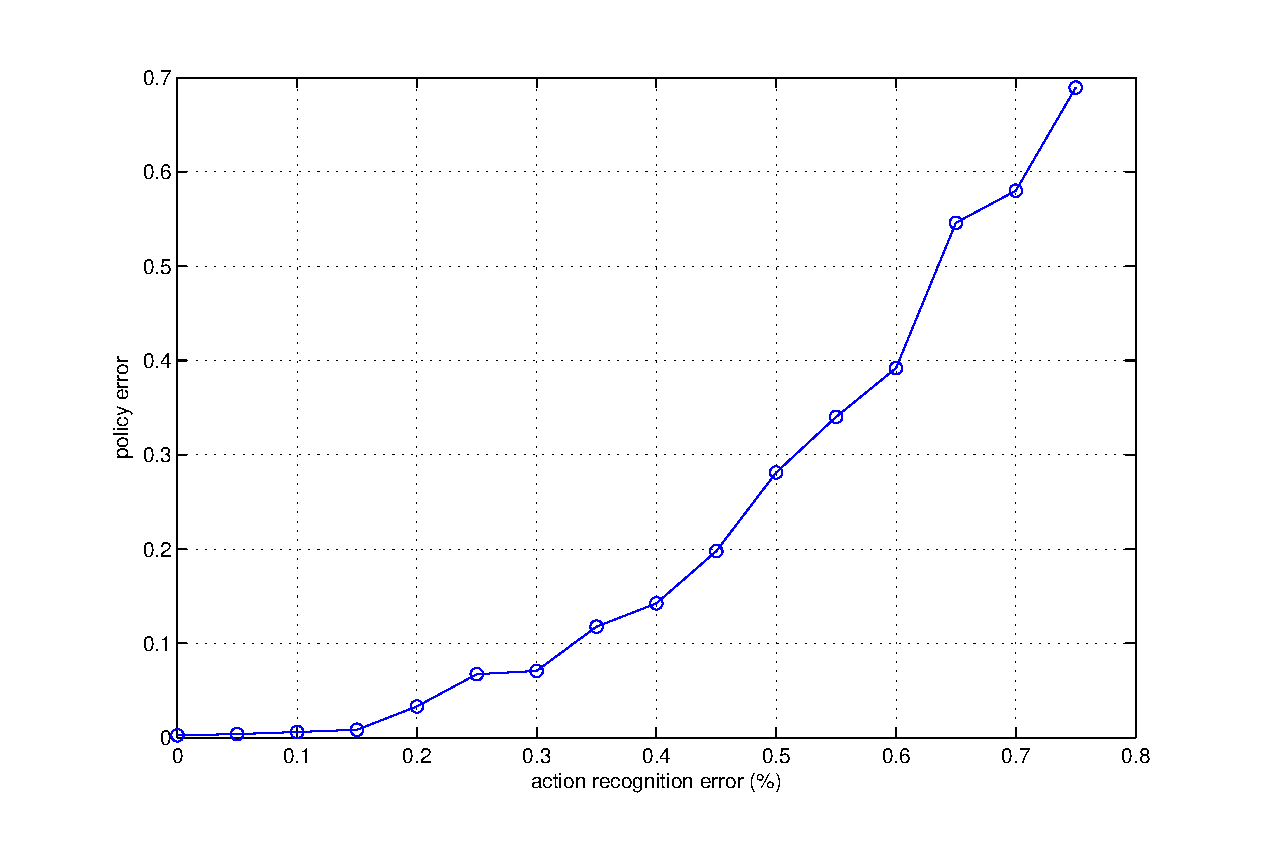
\includegraphics[width=0.45\columnwidth]{images/error.eps} \\
(a) & (b) \\
\end{tabular}
%Figure 7
\caption{Experimental evaluation: (a) setup for imitation learning of
  object sorting, (b) Percentage of wrong actions in the learnt policy
  as the action recognition errors increase.}
\label{fig:manipulation:experim}
\end{figure}

\endinput
